\section*{CHAPTER 4. OTFS WITH INDEX MODULATION DESIGN}
\addcontentsline{toc}{section}{CHAPTER 4. OTFS WITH INDEX MODULATION DESIGN}

% =========================================================
% Numbering for Chapter 4
% =========================================================
\setcounter{section}{4}
\setcounter{subsection}{0}
\setcounter{subsubsection}{0}
\setcounter{figure}{0}
\setcounter{table}{0}
\setcounter{equation}{0}

\renewcommand{\thefigure}{4.\arabic{figure}}
\renewcommand{\thetable}{4.\arabic{table}}
\renewcommand{\theequation}{4.\arabic{equation}}
\renewcommand{\theHfigure}{4.\arabic{figure}}
\renewcommand{\theHtable}{4.\arabic{table}}
\renewcommand{\theHequation}{4.\arabic{equation}}

% =========================================================
% Chapter Introduction
% =========================================================
This chapter extends the baseline OTFS system by introducing Index Modulation in the delay-Doppler domain. The focus is on the OTFS-IM block structure, activation-pattern mapping, spectral-efficiency trade-off, transmitter and receiver design, and the OHD-based pattern-selection methods used for the simulation study in Chapter 5. The design is motivated by prior work on OTFS-IM and efficient OTFS-IM detection~\cite{Liang2020OTFSIM,Wu2024OTFSIMDetector,Qian2022BlockWiseOTFSIM,Qian2023ReceiverOTFSIM}.

% =========================================================
% Chapter Sections
% =========================================================
\subsection{OTFS-IM Design Objectives and Architecture}

This section introduces the role of OTFS-IM in the proposed system design. It clarifies why index modulation is applied in the delay-Doppler domain and how the resulting architecture extends the baseline OTFS model.

\subsubsection{Motivation and Design Objectives}

The baseline OTFS system developed in Chapter 3 places QAM symbols on all available delay-Doppler resource elements. This structure is suitable for time-varying multipath channels because the information symbols are represented in a domain where delay and Doppler effects can be described more naturally. However, the baseline OTFS transmitter uses only the symbol values themselves to convey information. The positions of the delay-Doppler resource elements are fixed and do not carry additional bits.

Index Modulation introduces a different way of using the same resource grid. Instead of activating every resource element, only a selected subset of positions is activated inside each transmission block. The activation pattern itself represents part of the transmitted information, while the active positions still carry conventional modulation symbols. In OFDM-IM, this idea is applied to frequency-domain subcarriers. In OTFS-IM, the same principle is transferred to the delay-Doppler domain, where the active delay-Doppler positions become information-bearing indices.

The motivation for combining OTFS and IM is therefore twofold. First, OTFS provides a modulation framework suitable for high-Doppler and high-mobility channels. Second, IM provides an additional information-bearing dimension through activation patterns. This combination is particularly relevant when low-order modulation is used, because the loss caused by deactivating some positions can be compensated by the additional index bits. In the present thesis, 4-QAM is used for both the baseline OTFS and OTFS-IM systems, making the IM structure meaningful from a spectral-efficiency and reliability perspective.

The main design objective of the OTFS-IM system in this thesis is to evaluate how activation-pattern design affects performance under the same delay-Doppler channel model used for the baseline OTFS system. The goal is not merely to add inactive elements to the OTFS grid, but to construct a controlled OTFS-IM framework in which index bits, QAM symbol bits, and pattern-selection rules can be evaluated separately. For this reason, the later simulation results do not report only total BER. They also separate index BER, symbol BER, and pattern error rate, because these quantities explain whether the performance is limited by QAM symbol detection or by incorrect activation-pattern detection.

Another important objective is fairness. The OTFS-IM system is compared with the baseline OTFS system using the same delay-Doppler frame size, modulation order, channel-generation method, noise definition, and detector foundation. When an OTFS-IM configuration has the same spectral efficiency as the baseline OTFS system, its BER curve can be interpreted as a rate-fair comparison. When the spectral efficiency is lower, the result is interpreted as a reliability-oriented trade-off rather than a direct throughput advantage. This distinction is important because OTFS-IM does not automatically improve BER in every configuration; its benefit depends on the number of active positions, the selected pattern table, and the reliability of the receiver.

\subsubsection{Overall OTFS-IM Transceiver Architecture}

The overall OTFS-IM transceiver can be understood as an extension of the baseline OTFS chain. The OTFS modulation and demodulation blocks remain the same as in Chapter 3. The key difference appears before OTFS modulation and after delay-Doppler-domain detection. At the transmitter, an OTFS-IM mapper converts the input bit stream into two parts: index bits and QAM symbol bits. The index bits select an activation pattern from a predefined pattern table, while the QAM symbol bits are mapped to constellation symbols placed only on the active positions.

The resulting delay-Doppler grid contains both nonzero QAM symbols and zero-valued inactive elements. This is the most fundamental structural difference between OTFS and OTFS-IM. In conventional OTFS, every delay-Doppler position carries a modulation symbol. In OTFS-IM, the zero positions are intentional and meaningful: their locations help define the selected activation pattern. Consequently, the receiver must recover not only the values of the active QAM symbols but also the pattern of active and inactive positions.

After the OTFS-IM mapper constructs the delay-Doppler grid, the remaining transmitter operations follow the baseline OTFS modulation process. The grid is transformed to the time-frequency domain by the ISFFT operation and then converted to a time-domain transmit signal by the Heisenberg transform, or equivalently by the discrete implementation used in the simulation. The signal then passes through the same time-varying delay-Doppler channel model introduced in Chapter 3.

At the receiver, the signal is demodulated back to the delay-Doppler domain. The MP detector provides probability information for each resource element. In the baseline OTFS receiver, this probability information is mainly used to make hard QAM symbol decisions. In OTFS-IM, it has a more central role because the receiver must determine whether each position is active or inactive. The receiver therefore uses the MP output probabilities to perform block-wise pattern detection and QAM symbol detection.

At the discrete processing level, the input bits are first mapped into a vectorized delay-Doppler frame, where inactive positions are kept at zero and active positions contain scaled QAM symbols. The vector is reshaped into the delay-Doppler grid and passed through the common OTFS modulation block. After channel propagation and demodulation, the MP detector produces symbol probabilities. These probabilities are then processed block by block to choose the most likely activation pattern and the most likely QAM symbols.

\begin{figure}[H]
    \centering
    \resizebox{0.98\linewidth}{!}{
    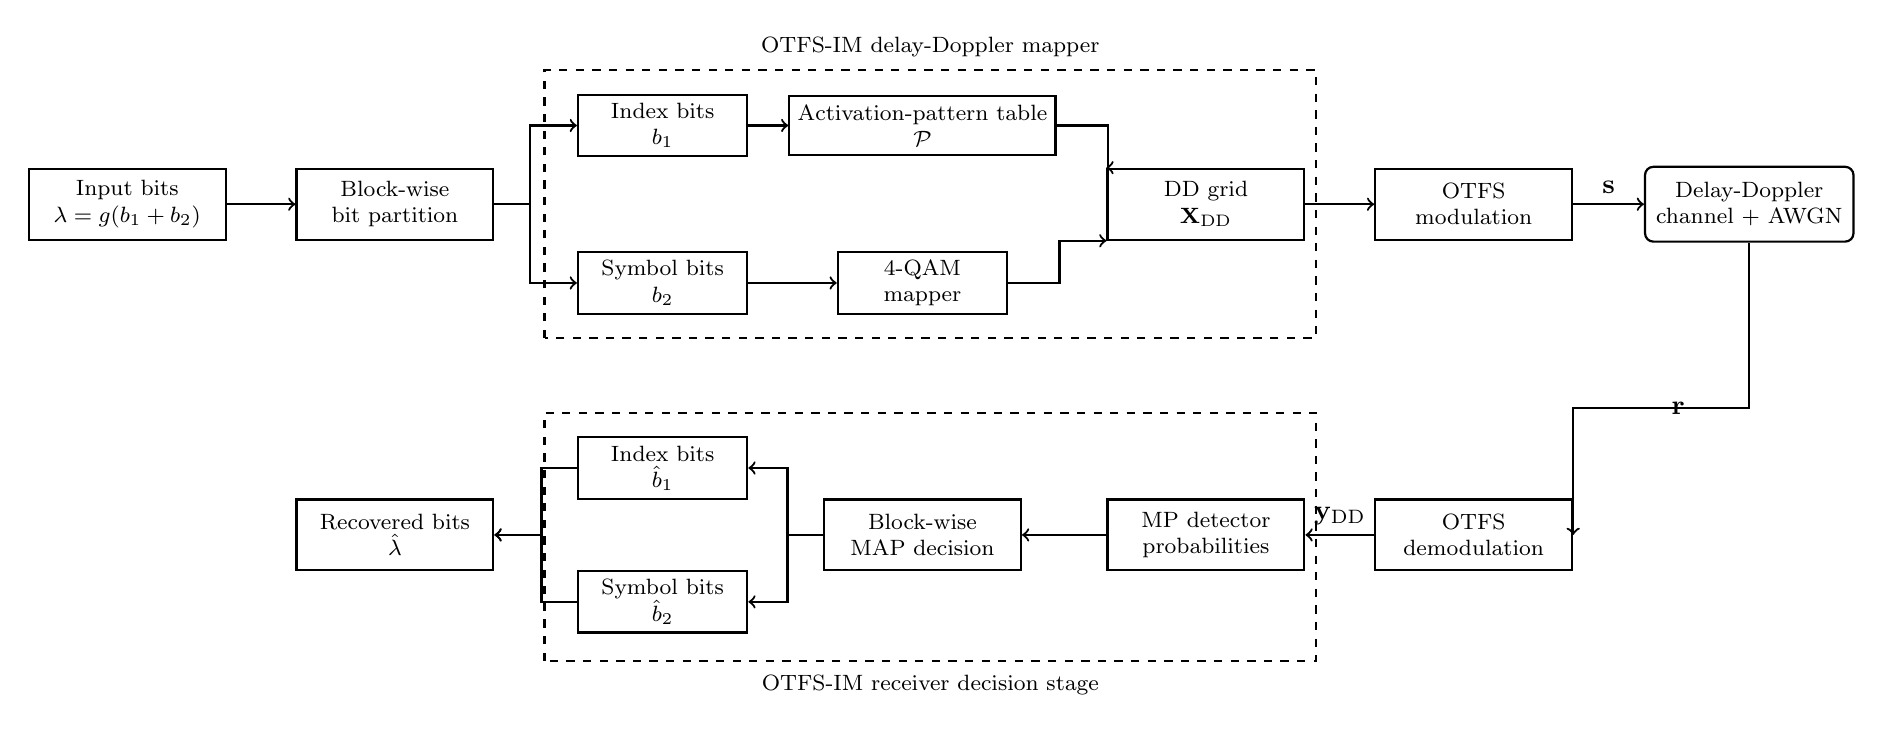
\begin{tikzpicture}[
        block/.style={
            rectangle,
            draw,
            thick,
            align=center,
            minimum width=2.5cm,
            minimum height=0.9cm,
            font=\footnotesize,
            inner sep=4pt
        },
        smallblock/.style={
            rectangle,
            draw,
            thick,
            align=center,
            minimum width=2.15cm,
            minimum height=0.75cm,
            font=\footnotesize,
            inner sep=3pt
        },
        channel/.style={
            rectangle,
            draw,
            thick,
            rounded corners=3pt,
            align=center,
            minimum width=2.6cm,
            minimum height=0.95cm,
            font=\footnotesize,
            inner sep=4pt
        },
        arrow/.style={->, thick}
    ]

        % Transmitter path
        \node[block] (inbits) at (0,0) {Input bits\\\(\lambda=g(b_1+b_2)\)};
        \node[block] (split) at (3.4,0) {Block-wise\\bit partition};
        \node[smallblock] (idx) at (6.8,1.0) {Index bits\\\(b_1\)};
        \node[smallblock] (sym) at (6.8,-1.0) {Symbol bits\\\(b_2\)};
        \node[smallblock] (map) at (10.1,1.0) {Activation-pattern table\\\(\mathcal{P}\)};
        \node[smallblock] (qam) at (10.1,-1.0) {4-QAM\\mapper};
        \node[block] (ddgrid) at (13.7,0) {DD grid\\\(\mathbf{X}_{\mathrm{DD}}\)};
        \node[block] (mod) at (17.1,0) {OTFS\\modulation};
        \node[channel] (chan) at (20.6,0) {Delay-Doppler\\channel + AWGN};

        % Receiver path
        \node[block] (demod) at (17.1,-4.2) {OTFS\\demodulation};
        \node[block] (mp) at (13.7,-4.2) {MP detector\\probabilities};
        \node[block] (mapdet) at (10.1,-4.2) {Block-wise\\MAP decision};
        \node[smallblock] (idxrx) at (6.8,-3.35) {Index bits\\\(\hat{b}_1\)};
        \node[smallblock] (symrx) at (6.8,-5.05) {Symbol bits\\\(\hat{b}_2\)};
        \node[block] (outbits) at (3.4,-4.2) {Recovered bits\\\(\hat{\lambda}\)};

        % Transmitter arrows
        \draw[arrow] (inbits.east) -- (split.west);
        \draw[arrow] (split.east) -- ++(0.45,0) |- (idx.west);
        \draw[arrow] (split.east) -- ++(0.45,0) |- (sym.west);
        \draw[arrow] (idx.east) -- (map.west);
        \draw[arrow] (sym.east) -- (qam.west);
        \draw[arrow] (map.east) -- ++(0.65,0) |- (ddgrid.north west);
        \draw[arrow] (qam.east) -- ++(0.65,0) |- (ddgrid.south west);
        \draw[arrow] (ddgrid.east) -- (mod.west);
        \draw[arrow] (mod.east) -- node[above] {\(\mathbf{s}\)} (chan.west);

        % Receiver arrows
        \draw[arrow] (chan.south) -- ++(0,-2.1) -| node[pos=0.25, right] {\(\mathbf{r}\)} (demod.east);
        \draw[arrow] (demod.west) -- node[above] {\(\mathbf{y}_{\mathrm{DD}}\)} (mp.east);
        \draw[arrow] (mp.west) -- (mapdet.east);
        \draw[arrow] (mapdet.west) -- ++(-0.45,0) |- (idxrx.east);
        \draw[arrow] (mapdet.west) -- ++(-0.45,0) |- (symrx.east);
        \draw[arrow] (idxrx.west) -- ++(-0.45,0) |- (outbits.east);
        \draw[arrow] (symrx.west) -- ++(-0.45,0) |- (outbits.east);

        \draw[dashed, thick] (5.3,-1.7) rectangle (15.1,1.7);
        \node[font=\footnotesize] at (10.2,2.0) {OTFS-IM delay-Doppler mapper};
        \draw[dashed, thick] (5.3,-5.8) rectangle (15.1,-2.65);
        \node[font=\footnotesize] at (10.2,-6.1) {OTFS-IM receiver decision stage};

    \end{tikzpicture}
    }
    \caption{Overall architecture of the implemented OTFS-IM transceiver}
    \label{fig:otfs_im_transceiver_architecture}
\end{figure}

\subsubsection{Design Scope and Relation to the Baseline OTFS System}

The OTFS-IM design in this chapter is built deliberately on top of the baseline OTFS system. The baseline system already defines the delay-Doppler grid, the modulation and demodulation operations, the channel model, and the MP detector. Chapter 4 therefore focuses only on the components that are new to OTFS-IM: block-wise mapping, activation-pattern tables, pattern selection, and block-wise receiver decisions.

This separation avoids unnecessary repetition. The ISFFT, Heisenberg transform, Wigner transform, SFFT, and delay-Doppler input-output model have already been developed in Chapter 3. In this chapter, these blocks are treated as established processing stages. The emphasis is instead placed on how the delay-Doppler input grid is constructed differently and how the receiver interprets the probability output of the detector differently.

The system considered in this thesis is an uncoded OTFS-IM system with perfect channel-state information at the receiver. Channel coding, channel estimation, synchronization errors, and standardized vehicular channel profiles are not included in the Chapter 4 design. These assumptions are consistent with the baseline model in Chapter 3 and are chosen to isolate the effect of index modulation and activation-pattern selection. Adding more practical impairments would make it harder to determine whether the observed performance difference comes from OTFS-IM itself or from another system component.

The design scope also differs from some OTFS-IM studies that focus mainly on new detector architectures such as MMSE-based or vector-wise message passing detectors. In this thesis, the receiver uses the existing MP detector as a probability engine and adds a block-wise MAP decision stage for OTFS-IM. This choice keeps the receiver structure close to the baseline OTFS system while still allowing the thesis to evaluate the reliability of index detection. The main contribution is therefore not a completely new OTFS detector, but a controlled OTFS-IM simulation framework with deterministic activation-pattern selection and detailed error-component analysis.

This design direction leads naturally to the rest of the chapter. Section 4.2 defines the IM block and spectral-efficiency calculation. Section 4.3 introduces the activation-pattern table. Section 4.4 describes the OTFS-IM transmitter. Section 4.5 presents the receiver and block-wise MAP detection process. Section 4.6 then develops the OHD and Balanced-OHD pattern-selection methods used to construct reliable activation-pattern tables.


\subsection{Index Modulation Block and Spectral Efficiency}

This section defines the OTFS-IM block structure used in the thesis and relates the mathematical parameters to the simulation model. Unlike Chapter 2, where IM was introduced as a general principle, this section focuses on how index modulation is embedded into the \(N \times M\) delay-Doppler grid of the implemented OTFS-IM system.

\subsubsection{Delay-Doppler IM Block Structure}

In the baseline OTFS system, all \(NM\) delay-Doppler resource elements are occupied by QAM symbols. In OTFS-IM, the same delay-Doppler frame is divided into smaller index-modulation blocks. Each block contains \(n\) delay-Doppler positions, of which only \(k\) positions are active. The remaining \(n-k\) positions are set to zero and are interpreted as inactive positions.

Let \(N\) denote the number of Doppler bins and \(M\) denote the number of delay bins. The total number of delay-Doppler resource elements in one OTFS frame is
\begin{equation}
    N_{\mathrm{total}} = NM .
\end{equation}
The OTFS-IM block size \(n\) is chosen such that it divides \(NM\), so that the frame can be partitioned into an integer number of IM blocks. The number of IM blocks per OTFS frame is therefore
\begin{equation}
    g = \frac{NM}{n}.
    \label{eq:otfs_im_num_blocks}
\end{equation}
The block partitioning is applied to the vectorized delay-Doppler grid. The transmit vector \(\mathbf{x}_{\mathrm{vec}}\) has length \(NM\). For the \(i\)-th IM block, the positions from \((i-1)n+1\) to \(in\) form one local activation block. The active positions inside this block are determined by the selected activation pattern, while all inactive positions remain zero.

This block-wise construction is important for two reasons. First, it defines how the input bit sequence is mapped to the delay-Doppler grid. Second, it limits the receiver search to a small block rather than the entire OTFS frame. Without this block structure, detecting the active-position pattern over all \(NM\) resource elements would be computationally impractical.

\subsubsection{Bit Partitioning and Activation Patterns}

Each OTFS-IM block carries information in two parts. The first part is represented by the activation pattern, and the second part is represented by QAM symbols transmitted on the active positions. For a block with \(n\) available positions and \(k\) active positions, the number of possible constant-weight activation patterns is \(\binom{n}{k}\). Since binary mapping requires a power-of-two number of labels, the number of index bits per block is
\begin{equation}
    b_1 =
    \left\lfloor
    \log_2 \binom{n}{k}
    \right\rfloor .
    \label{eq:otfs_im_index_bits}
\end{equation}
Only \(2^{b_1}\) patterns are selected and stored in the activation-pattern table, denoted by \(\mathcal{P}\). This table will be discussed in more detail in Section 4.3.

The second part of each block consists of QAM symbol bits. Since only \(k\) positions are active and each active position carries one \(M_{\mathrm{mod}}\)-ary QAM symbol, the number of QAM symbol bits per IM block is
\begin{equation}
    b_2 = k\log_2(M_{\mathrm{mod}}).
    \label{eq:otfs_im_symbol_bits}
\end{equation}
In this thesis, \(M_{\mathrm{mod}}=4\), so each active resource element carries two QAM bits.

Therefore, the total number of information bits per OTFS-IM block is
\begin{equation}
    b_{\mathrm{block}} = b_1 + b_2.
    \label{eq:otfs_im_bits_per_block}
\end{equation}
For one full OTFS-IM frame, the total number of transmitted bits is
\begin{equation}
    \lambda = g(b_1+b_2).
    \label{eq:otfs_im_total_bits}
\end{equation}
For each OTFS-IM frame, a binary vector of length \(\lambda\) is generated. The receiver reconstructs a vector of the same length after block-wise pattern and symbol detection.

Table~\ref{tab:otfs_im_parameters} summarizes the main OTFS-IM block parameters used in the simulation. This table is useful because Chapter 5 changes \((n,k)\) to compare different spectral-efficiency and reliability trade-offs.

\begin{table}[H]
\centering
\caption{Main OTFS-IM block parameters used in the simulation.}
\label{tab:otfs_im_parameters}
\begin{tabularx}{0.95\linewidth}{|c|c|X|}
\hline
\textbf{Symbol} & \textbf{Simulation parameter} & \textbf{Meaning} \\
\hline
\(N\) & Doppler-bin count & Number of Doppler bins in one OTFS frame. \\
\hline
\(M\) & Delay-bin count & Number of delay bins in one OTFS frame. \\
\hline
\(NM\) & Total DD resources & Total number of delay-Doppler resource elements. \\
\hline
\(n\) & IM block length & Number of resource elements in one IM block. \\
\hline
\(k\) & Active positions per block & Number of active resource elements in one IM block. \\
\hline
\(g\) & Number of IM blocks & Number of IM blocks per OTFS frame. \\
\hline
\(b_1\) & Index-bit count & Number of index bits per IM block. \\
\hline
\(b_2\) & Symbol-bit count & Number of QAM symbol bits per IM block. \\
\hline
\(\lambda\) & Frame bit length & Total number of transmitted bits per OTFS-IM frame. \\
\hline
\end{tabularx}
\end{table}

\subsubsection{Spectral Efficiency and Power Normalization}

The spectral efficiency of the baseline OTFS system is straightforward because every delay-Doppler resource element carries one QAM symbol. With \(M_{\mathrm{mod}}\)-ary QAM, the baseline OTFS spectral efficiency is
\begin{equation}
    \eta_{\mathrm{OTFS}} = \log_2(M_{\mathrm{mod}}).
    \label{eq:otfs_baseline_se}
\end{equation}
For 4-QAM, \(\eta_{\mathrm{OTFS}} = 2\) bits per delay-Doppler resource element.

For OTFS-IM, the spectral efficiency is determined by the number of transmitted bits per frame divided by the number of delay-Doppler resource elements:
\begin{equation}
    \eta_{\mathrm{IM}}
    =
    \frac{\lambda}{NM}
    =
    \frac{g(b_1+b_2)}{NM}.
    \label{eq:otfs_im_se_frame}
\end{equation}
Using \(g = NM/n\), this can also be written as
\begin{equation}
    \eta_{\mathrm{IM}}
    =
    \frac{b_1+b_2}{n}
    =
    \frac{
    \left\lfloor \log_2 \binom{n}{k} \right\rfloor
    +
    k\log_2(M_{\mathrm{mod}})
    }{n}.
    \label{eq:otfs_im_se_block}
\end{equation}
This expression is the spectral-efficiency value used to compare different OTFS-IM configurations.

Power normalization is also required because only \(k\) out of \(n\) positions are active in each IM block. If the active QAM symbols were transmitted without scaling, the average block energy would decrease simply because some positions are set to zero. To keep the energy comparison controlled, the active symbols are scaled by
\begin{equation}
    \alpha = \sqrt{\frac{n}{k}}.
    \label{eq:otfs_im_alpha}
\end{equation}
In the transmitter, the QAM symbols on active positions are multiplied by \(\alpha\). At the receiver, the demodulated delay-Doppler grid is divided by \(\alpha\), and the noise variance used by the detector is adjusted by \(\alpha^2\).

The normalization does not remove the detection difficulty of OTFS-IM. The receiver still has to distinguish active and inactive positions under noise and channel interference. Rather, the purpose of \(\alpha\) is to prevent the BER comparison from being dominated by a trivial transmit-energy mismatch between OTFS and OTFS-IM.

\subsubsection{Rate-Fair and Reliability-Oriented Configurations}

The choice of \(n\) and \(k\) determines the operating point of the OTFS-IM system. A configuration is considered rate-fair with the baseline OTFS system when
\begin{equation}
    \eta_{\mathrm{IM}} = \eta_{\mathrm{OTFS}}.
\end{equation}
Under this condition, BER curves can be compared directly because both systems transmit the same number of bits per delay-Doppler resource element.

For example, with 4-QAM and \((n,k)=(4,3)\),
\begin{equation}
    b_1 = \left\lfloor \log_2 \binom{4}{3} \right\rfloor = 2,
    \qquad
    b_2 = 3\log_2(4)=6,
\end{equation}
so that
\begin{equation}
    \eta_{\mathrm{IM}} = \frac{2+6}{4}=2
    \ \text{bits/resource element}.
\end{equation}
This is equal to the baseline OTFS spectral efficiency with 4-QAM.

Another useful equal-rate example is \((n,k)=(5,4)\). In this case,
\begin{equation}
    b_1 = \left\lfloor \log_2 \binom{5}{4} \right\rfloor = 2,
    \qquad
    b_2 = 4\log_2(4)=8,
\end{equation}
and therefore
\begin{equation}
    \eta_{\mathrm{IM}} = \frac{2+8}{5}=2
    \ \text{bits/resource element}.
\end{equation}
This configuration is also consistent with the common IM design guideline that, for low-order modulation, the number of active positions should be a large fraction of the block size when spectral efficiency is the priority.

In contrast, configurations such as \((n,k)=(4,2)\) have lower spectral efficiency:
\begin{equation}
    b_1 = \left\lfloor \log_2 \binom{4}{2} \right\rfloor = 2,
    \qquad
    b_2 = 2\log_2(4)=4,
\end{equation}
which gives
\begin{equation}
    \eta_{\mathrm{IM}} = \frac{2+4}{4}=1.5
    \ \text{bits/resource element}.
\end{equation}
Such a configuration should not be interpreted as a direct rate-fair BER comparison against baseline OTFS. Instead, it represents a reliability-oriented operating point where the system sacrifices spectral efficiency in exchange for a potentially easier detection problem.

Table~\ref{tab:otfs_im_config_examples} lists representative OTFS-IM configurations used or considered in the simulation study. The table also indicates how the corresponding results should be interpreted.

\begin{table}[H]
\centering
\caption{Representative OTFS-IM configurations and interpretation.}
\label{tab:otfs_im_config_examples}
\begin{tabular}{|c|c|c|c|c|}
\hline
\(\boldsymbol{n}\) & \(\boldsymbol{k}\) & \(\boldsymbol{b_1}\) & \(\boldsymbol{\eta_{\mathrm{IM}}}\) & \textbf{Interpretation} \\
\hline
4 & 2 & 2 & 1.50 & Reliability-oriented lower-rate case \\
\hline
4 & 3 & 2 & 2.00 & Rate-fair comparison with 4-QAM OTFS \\
\hline
5 & 4 & 2 & 2.00 & Rate-fair comparison with high active ratio \\
\hline
6 & 4 & 3 & 1.83 & Supplementary BER-SE trade-off case \\
\hline
6 & 5 & 2 & 2.00 & Rate-fair high-active-ratio validation \\
\hline
\end{tabular}
\end{table}

The selected configurations therefore serve different purposes. Rate-fair configurations are used to compare OTFS and OTFS-IM under the same spectral efficiency. Lower-rate configurations are useful for studying whether reducing the number of active positions improves the reliability of pattern and symbol detection. This distinction is carried into Chapter 5, where BER, index BER, symbol BER, and pattern error rate are interpreted together rather than relying on total BER alone.


\subsection{Activation Pattern Table Design}

After the OTFS-IM block parameters have been defined, the next design step is to determine how the index bits are converted into active delay-Doppler positions. This section describes the activation-pattern table used by the transmitter and receiver. The purpose is not only to list possible patterns, but also to explain why the pattern table has a direct influence on index detection reliability.

\subsubsection{Constant-Weight Pattern Table}

In each OTFS-IM block, exactly \(k\) out of \(n\) delay-Doppler positions are active. Therefore, every valid activation pattern has the same Hamming weight \(k\). The complete set of possible activation patterns is generated by choosing \(k\) positions from \(n\) available positions:
\begin{equation}
    \mathcal{A}_{\mathrm{all}}
    =
    \left\{
    \mathbf{a} \in \{0,1\}^{n}
    :
    \sum_{i=1}^{n} a_i = k
    \right\}.
    \label{eq:all_constant_weight_patterns}
\end{equation}
The number of candidate patterns is \(\binom{n}{k}\). Each candidate can be stored either as a set of active positions or as a binary vector. For example, when \(n=4\) and \(k=3\), a pattern row \([1,2,4]\) means that the first, second, and fourth positions in the local IM block are active, while the third position is inactive.

For distance evaluation, the position-index representation is converted into a binary vector representation. If the active positions are \([1,2,4]\), the corresponding binary pattern is
\begin{equation}
    \mathbf{a} = [1,1,0,1].
\end{equation}
This binary representation is useful because the difference between two activation patterns can be measured directly by their Hamming distance.

Although \(\binom{n}{k}\) patterns may be available, not all of them are necessarily used. The number of index bits per block is
\begin{equation}
    b_1 =
    \left\lfloor
    \log_2 \binom{n}{k}
    \right\rfloor ,
\end{equation}
so only \(2^{b_1}\) patterns can be assigned to binary input labels. The selected pattern table is denoted by
\begin{equation}
    \mathcal{P}
    =
    \left\{
    \mathbf{p}_0, \mathbf{p}_1, \ldots, \mathbf{p}_{2^{b_1}-1}
    \right\},
    \label{eq:selected_pattern_table}
\end{equation}
This table is shared by the transmitter and receiver. The transmitter uses it to decide which delay-Doppler positions are active, while the receiver uses the same table as the set of candidate patterns in the block-wise detection process.

\subsubsection{Index-to-Pattern Mapping}

In each IM block, the first \(b_1\) bits are interpreted as index bits. These bits are converted into a decimal index and then mapped to one row of the selected table \(\mathcal{P}\). The binary index is first obtained as
\begin{equation}
    q =
    \mathrm{bin2dec}
    \left(
    \mathbf{b}_{\mathrm{idx}}
    \right),
    \qquad
    q \in \{0,1,\ldots,2^{b_1}-1\}.
    \label{eq:index_binary_decimal}
\end{equation}
The simulation then applies Gray indexing before selecting the pattern row:
\begin{equation}
    m = q \oplus \left\lfloor \frac{q}{2} \right\rfloor ,
    \label{eq:gray_index_mapping}
\end{equation}
where \(\oplus\) denotes bitwise exclusive-or. The active positions for the current block are then read from
\begin{equation}
    \mathbf{p}_m = \mathcal{P}[m].
\end{equation}

For the \(i\)-th IM block, the local active positions \(\mathbf{p}_m\) are shifted to the corresponding positions in the vectorized delay-Doppler frame. The QAM symbols are inserted only at these active locations, while the other positions in the same block remain zero. Therefore, the transmitted block carries information through both the selected pattern and the QAM symbols placed on the active positions.

At the receiver, the same pattern table is used in the reverse direction. The detector evaluates every candidate row of \(\mathcal{P}\) and selects the pattern that gives the largest likelihood score. After the most likely Gray index is found, it is converted back to the original binary index bits. This ensures that the transmitter and receiver use a consistent mapping between index bits and activation patterns.

The use of a fixed pattern table is important for reproducibility. If the transmitter and receiver used different pattern ordering, the active positions might still be detected correctly but the recovered index bits would be wrong. Therefore, the pattern table must be treated as part of the system design rather than as a temporary implementation detail.

\subsubsection{Pattern-Distance Interpretation and Selection Need}

The reliability of index detection depends strongly on how distinguishable the selected activation patterns are. Two patterns that differ in only a small number of positions are more likely to be confused after channel distortion, noise, and imperfect probability estimation. This effect is measured by the Hamming distance between two binary patterns:
\begin{equation}
    d_{\mathrm{H}}(\mathbf{p}_i,\mathbf{p}_j)
    =
    \sum_{\ell=1}^{n}
    \left|
    p_i(\ell) - p_j(\ell)
    \right| .
    \label{eq:pattern_hamming_distance}
\end{equation}
For constant-weight patterns, the Hamming distance counts how many local block positions change their active or inactive status between two candidate patterns. A larger Hamming distance generally means that the receiver must make more activation-position mistakes before one pattern is confused with another.

The minimum pairwise Hamming distance of a selected pattern table is defined as
\begin{equation}
    d_{\min}
    =
    \min_{i \ne j}
    d_{\mathrm{H}}(\mathbf{p}_i,\mathbf{p}_j).
    \label{eq:pattern_min_distance}
\end{equation}
This metric is useful because the worst-separated pair of patterns often dominates the pattern error behavior. If two patterns in the table are too similar, a small detection error in one delay-Doppler position can cause an incorrect index decision.

However, maximizing only the number of possible patterns is not always the best design choice. Since only \(2^{b_1}\) patterns are used, the system has an opportunity to select a subset with better distance properties. This is the motivation for the OHD-based pattern selection methods discussed later in Section 4.6. In the present section, the important point is that \(\mathcal{P}\) is not merely a lookup table for implementation convenience. It determines the geometric separation among index labels and therefore affects index BER, pattern error rate, and total OTFS-IM BER.

In the simulation results of Chapter 5, this effect is evaluated by comparing different pattern-selection methods under the same \((n,k)\), modulation order, and channel setting. The total BER alone is not sufficient to explain the role of the activation table, so index BER and pattern error rate are also reported. These additional metrics reveal whether performance changes come from symbol detection errors or from incorrect activation-pattern decisions.


\subsection{OTFS-IM Transmitter Design}

This section describes how the OTFS-IM transmitter constructs the delay-Doppler input grid used by the common OTFS modulation block. Compared with the baseline OTFS transmitter in Chapter 3, the new operation is the block-wise mapping from input bits to activation patterns and active QAM symbols. After the OTFS-IM grid is formed, the ISFFT and Heisenberg transform are reused without structural modification.

\subsubsection{Overview of the OTFS-IM Transmitter Processing Chain}

The transmitter starts from a binary vector of length \(\lambda\), where
\begin{equation}
    \lambda = g(b_1+b_2).
\end{equation}
This vector is processed block by block. In each block, the first \(b_1\) bits select the activation pattern, while the following \(b_2\) bits are mapped to QAM symbols. Only the selected active positions are filled with QAM symbols; all other positions remain zero.

Figure~\ref{fig:otfs_im_transmitter_flow} summarizes the implemented transmitter processing flow. The purpose of the figure is to show the internal OTFS-IM mapping stage before the standard OTFS modulation block is applied.

\begin{figure}[H]
    \centering
    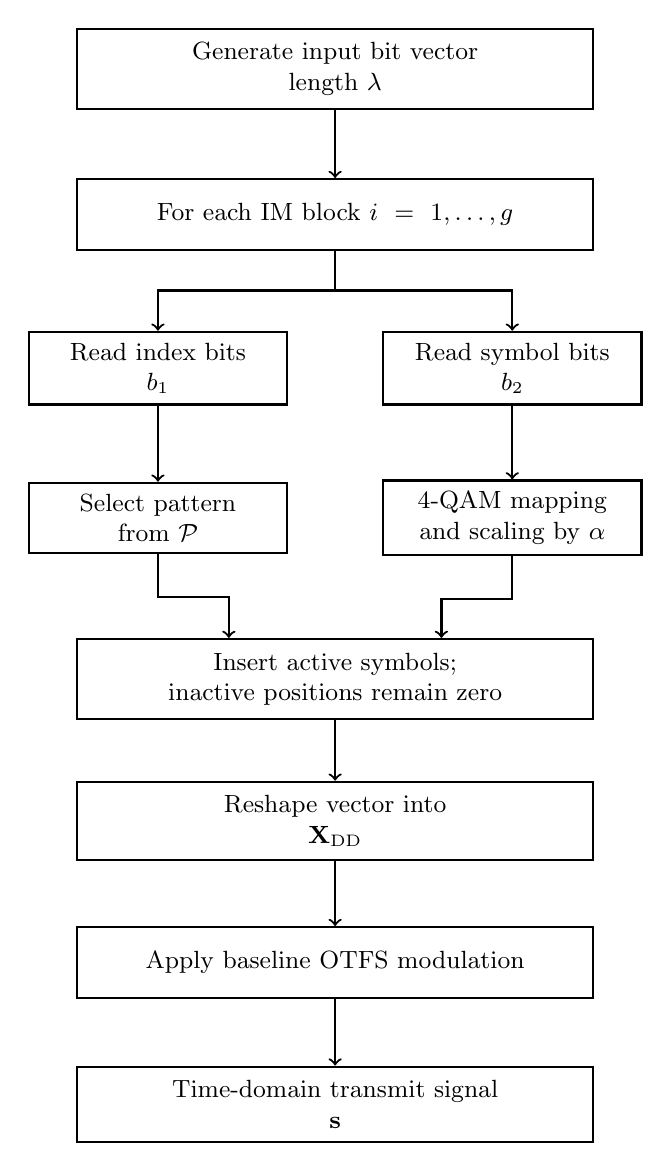
\begin{tikzpicture}[
        block/.style={
            rectangle,
            draw,
            thick,
            align=center,
            text width=6.2cm,
            minimum height=0.9cm,
            font=\small,
            inner sep=5pt
        },
        smallblock/.style={
            rectangle,
            draw,
            thick,
            align=center,
            text width=3.0cm,
            minimum height=0.85cm,
            font=\small,
            inner sep=4pt
        },
        arrow/.style={->, thick}
    ]

        \node[block] (bits) at (0,0) {Generate input bit vector\\length \(\lambda\)};
        \node[block] (loop) at (0,-1.85) {For each IM block \(i=1,\ldots,g\)};
        \node[smallblock] (idx) at (-2.25,-3.8) {Read index bits\\\(b_1\)};
        \node[smallblock] (sym) at (2.25,-3.8) {Read symbol bits\\\(b_2\)};
        \node[smallblock] (pat) at (-2.25,-5.7) {Select pattern\\from \(\mathcal{P}\)};
        \node[smallblock] (qam) at (2.25,-5.7) {4-QAM mapping\\and scaling by \(\alpha\)};
        \node[block] (insert) at (0,-7.75) {Insert active symbols;\\inactive positions remain zero};
        \node[block] (reshape) at (0,-9.55) {Reshape vector into\\\(\mathbf{X}_{\mathrm{DD}}\)};
        \node[block] (otfs) at (0,-11.35) {Apply baseline OTFS modulation};
        \node[block] (tx) at (0,-13.15) {Time-domain transmit signal\\\(\mathbf{s}\)};

        \draw[arrow] (bits.south) -- (loop.north);
        \draw[arrow] (loop.south) -- ++(0,-0.5) -| (idx.north);
        \draw[arrow] (loop.south) -- ++(0,-0.5) -| (sym.north);
        \draw[arrow] (idx.south) -- (pat.north);
        \draw[arrow] (sym.south) -- (qam.north);
        \draw[arrow] (pat.south) -- ++(0,-0.55) -| ([xshift=-1.35cm]insert.north);
        \draw[arrow] (qam.south) -- ++(0,-0.55) -| ([xshift=1.35cm]insert.north);
        \draw[arrow] (insert.south) -- (reshape.north);
        \draw[arrow] (reshape.south) -- (otfs.north);
        \draw[arrow] (otfs.south) -- (tx.north);

    \end{tikzpicture}
    \caption{OTFS-IM transmitter processing flow}
    \label{fig:otfs_im_transmitter_flow}
\end{figure}

This flow also reflects the separation between the proposed OTFS-IM mapping and the baseline OTFS modulation. The index-modulation part determines the sparse delay-Doppler grid, while the modulation part converts this grid into the transmitted time-domain waveform.

\subsubsection{Index and Symbol Bit Mapping}

For the \(i\)-th IM block, the transmitter reads \(b_1\) index bits and converts them into a decimal value. Let this value be denoted by \(q_i\). The implemented mapping then converts \(q_i\) into a Gray index:
\begin{equation}
    m_i
    =
    q_i
    \oplus
    \left\lfloor
    \frac{q_i}{2}
    \right\rfloor ,
    \label{eq:tx_gray_index}
\end{equation}
where \(\oplus\) denotes bitwise exclusive-or.
The selected activation pattern is then obtained from the pattern table:
\begin{equation}
    \mathbf{p}_{m_i}
    =
    \mathcal{P}[m_i].
    \label{eq:tx_pattern_selection}
\end{equation}
The entries of \(\mathbf{p}_{m_i}\) are local active positions inside the current IM block.

The next \(b_2\) bits are used to generate the active QAM symbols. Since
\begin{equation}
    b_2 = k\log_2(M_{\mathrm{mod}}),
\end{equation}
these bits form exactly \(k\) modulation symbols. In this thesis, \(M_{\mathrm{mod}}=4\), so each active position carries one 4-QAM symbol. The generated QAM symbols are multiplied by the normalization factor
\begin{equation}
    \alpha = \sqrt{\frac{n}{k}},
\end{equation}
which preserves the average block energy when only \(k\) out of \(n\) positions are active.

After one IM block is processed, the bit-reading position is advanced by \(b_1+b_2\) bits. This ensures that the input vector is consumed sequentially and that each block carries one index label and \(k\) active QAM symbols.

\subsubsection{Illustrative Block-Mapping Example}

To clarify the mapping process, consider the representative configuration \((n,k)=(4,3)\) with 4-QAM. In this case, there are
\begin{equation}
    \binom{4}{3}=4
\end{equation}
valid constant-weight activation patterns. Therefore,
\begin{equation}
    b_1=\left\lfloor \log_2 4 \right\rfloor=2,
    \qquad
    b_2=3\log_2(4)=6.
\end{equation}
Each IM block carries \(b_1+b_2=8\) information bits. The first two bits select one activation pattern, and the next six bits generate three 4-QAM symbols.

Suppose that the selected activation pattern is
\begin{equation}
    \mathbf{p}_{m_i}=[1,2,4].
\end{equation}
Then the first, second, and fourth local positions of the IM block are active, while the third local position is inactive. If the three scaled QAM symbols for this block are denoted by \(\alpha s_{i,1}\), \(\alpha s_{i,2}\), and \(\alpha s_{i,3}\), the local block vector becomes
\begin{equation}
    \mathbf{x}_{i}
    =
    \left[
    \alpha s_{i,1},
    \alpha s_{i,2},
    0,
    \alpha s_{i,3}
    \right]^{T}.
    \label{eq:otfs_im_local_block_example}
\end{equation}
This example shows the two-layer information structure of OTFS-IM. The nonzero symbol values carry QAM information, while the zero position carries index information because its location is part of the selected activation pattern.

For the next IM block, the same procedure is repeated on the next group of \(n\) delay-Doppler positions. Thus, the full OTFS-IM frame is not one arbitrary sparse vector. It is a structured sparse vector formed by concatenating \(g\) local IM blocks, each of which has exactly \(k\) active positions. This structure is what makes block-wise MAP detection possible at the receiver.

\subsubsection{Delay-Doppler Grid Construction}

The vectorized OTFS-IM delay-Doppler frame is denoted by \(\mathbf{x}_{\mathrm{vec}}\). It has length \(NM\) and is initialized as an all-zero vector:
\begin{equation}
    \mathbf{x}_{\mathrm{vec}} \in \mathbb{C}^{NM \times 1}.
\end{equation}
For the \(i\)-th IM block, the local positions are
\begin{equation}
    \mathcal{B}_i
    =
    \{(i-1)n+1,\ldots,in\}.
\end{equation}
If the selected local active pattern is \(\mathbf{p}_{m_i}\), then the global active positions are
\begin{equation}
    (i-1)n + \mathbf{p}_{m_i}.
    \label{eq:tx_global_active_positions}
\end{equation}
Only these positions are filled with the scaled QAM symbols. In compact form, the assignment can be written as
\begin{equation}
    \mathbf{x}_{\mathrm{vec}}\big((i-1)n+\mathbf{p}_{m_i}\big)
    =
    \alpha \mathbf{s}_i,
    \label{eq:tx_xvec_assignment}
\end{equation}
where \(\mathbf{s}_i\) contains the \(k\) QAM symbols of the \(i\)-th IM block.

All inactive positions remain zero by construction. This choice is simple but important: zeros are not missing symbols; they are intentional inactive resource elements that carry index information through their locations.

After all \(g\) IM blocks have been processed, the vector \(\mathbf{x}_{\mathrm{vec}}\) is reshaped into the \(N \times M\) delay-Doppler grid:
\begin{equation}
    \mathbf{X}_{\mathrm{DD}}
    =
    \mathrm{reshape}
    \left(
    \mathbf{x}_{\mathrm{vec}}, N, M
    \right).
    \label{eq:tx_xdd_reshape}
\end{equation}
This grid is the OTFS-IM counterpart of the full QAM delay-Doppler grid used in the baseline OTFS transmitter. The difference is that \(\mathbf{X}_{\mathrm{DD}}\) now contains both active QAM entries and inactive zero entries.

\subsubsection{Connection to the Baseline OTFS Modulation Block}

Once the OTFS-IM delay-Doppler grid has been constructed, the remaining modulation process is identical to the baseline OTFS transmitter. The OTFS-IM transmit signal can be written compactly as
\begin{equation}
    \mathbf{s}_{\mathrm{IM}}
    =
    \mathcal{M}_{\mathrm{OTFS}}
    \left\{
    \mathbf{X}_{\mathrm{DD}}
    \right\},
    \label{eq:otfs_im_common_modulation}
\end{equation}
where \(\mathcal{M}_{\mathrm{OTFS}}\{\cdot\}\) denotes the common OTFS modulation operation. The delay-Doppler grid is first transformed into the time-frequency domain using the ISFFT operation, and the time-domain transmit signal is then obtained through the discrete Heisenberg transform. Therefore, the transmitter design in this chapter does not redefine the OTFS modulation theory from Chapter 3. Instead, it changes the content of the delay-Doppler input grid before the common OTFS modulation block is applied.

This modular structure is useful for a fair comparison. Baseline OTFS and OTFS-IM share the same frame size, channel model, OTFS modulation and demodulation operations, and detector foundation. The main difference is the delay-Doppler grid construction. Consequently, the simulation results in Chapter 5 can attribute performance differences mainly to the use of index modulation and activation-pattern design rather than to a different physical-layer waveform implementation.


\subsection{OTFS-IM Receiver and Block-Wise MAP Detection}

The OTFS-IM receiver differs from the baseline OTFS receiver because it must recover both the active-position pattern and the QAM symbols placed on the active positions. Therefore, a hard symbol-by-symbol decision is not sufficient. In this thesis, the MP detector is used as a probability engine, and an additional block-wise MAP decision stage is applied to recover the index bits and symbol bits of each IM block.

\subsubsection{Overview of the OTFS-IM Receiver Processing Chain}

After transmission through the delay-Doppler channel, the received time-domain signal is demodulated by the same OTFS demodulation block used in Chapter 3. The output is a delay-Doppler-domain observation denoted by \(\mathbf{Y}_{\mathrm{DD}}\). Since the OTFS-IM transmitter scales active symbols by \(\alpha\), the receiver first normalizes the demodulated grid and the corresponding noise variance:
\begin{equation}
    \mathbf{Y}_{\mathrm{norm}}
    =
    \frac{\mathbf{Y}_{\mathrm{DD}}}{\alpha},
    \qquad
    \sigma^2_{\mathrm{norm}}
    =
    \frac{\sigma^2_{\mathrm{IM}}}{\alpha^2}.
    \label{eq:otfs_im_receiver_normalization}
\end{equation}
The normalized delay-Doppler grid is then passed to the MP detector. The detector estimates, for each delay-Doppler position, the probability that the transmitted value belongs to one of the QAM constellation points or to the inactive value zero. These probabilities are then used by the block-wise MAP stage to decide the most likely activation pattern and active QAM symbols.

Figure~\ref{fig:otfs_im_receiver_flow} summarizes the implemented OTFS-IM receiver flow.

\begin{figure}[H]
    \centering
    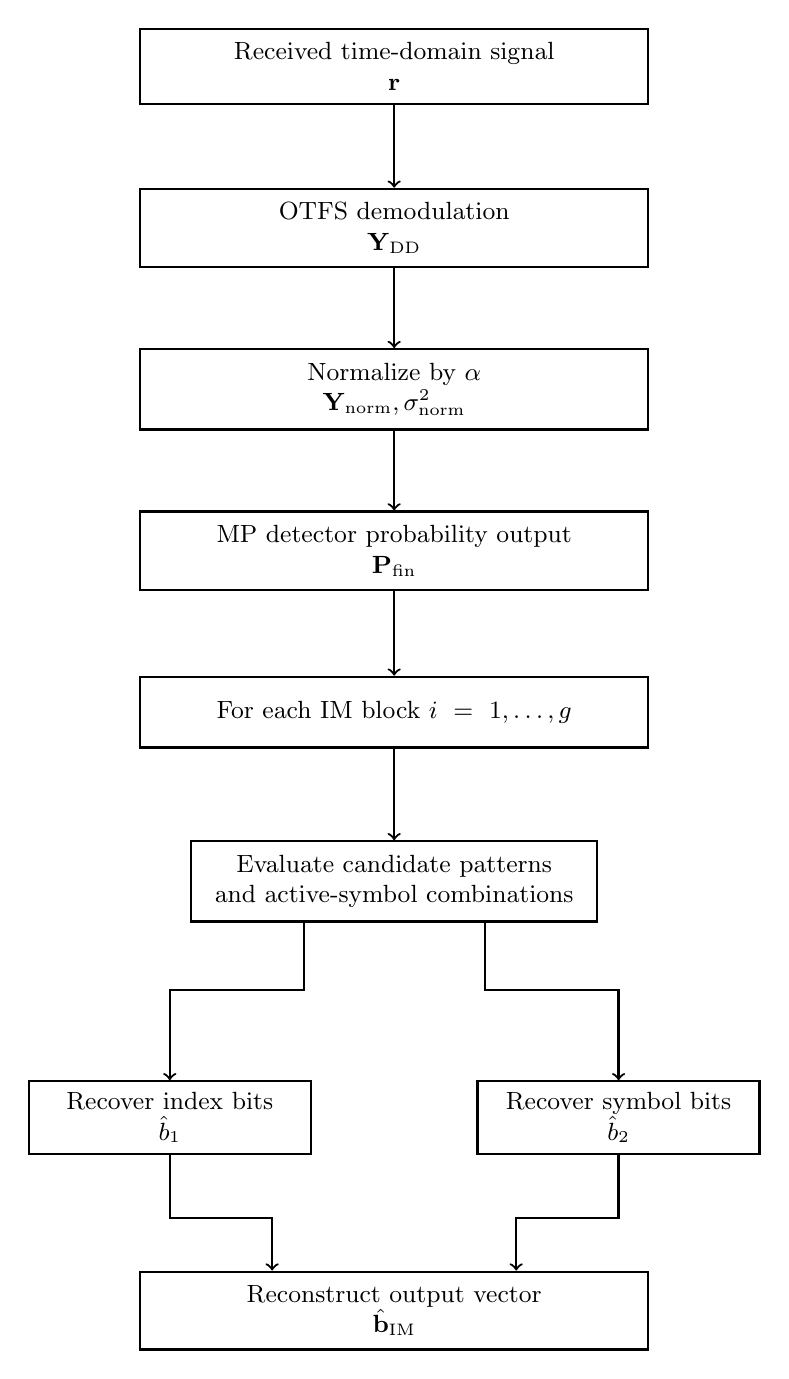
\begin{tikzpicture}[
        block/.style={
            rectangle,
            draw,
            thick,
            align=center,
            text width=6.1cm,
            minimum height=0.9cm,
            font=\small,
            inner sep=5pt
        },
        smallblock/.style={
            rectangle,
            draw,
            thick,
            align=center,
            text width=3.3cm,
            minimum height=0.85cm,
            font=\small,
            inner sep=4pt
        },
        scoreblock/.style={
            rectangle,
            draw,
            thick,
            align=center,
            text width=4.8cm,
            minimum height=0.9cm,
            font=\small,
            inner sep=5pt
        },
        arrow/.style={->, thick}
    ]

        \node[block] (rx) at (0,0) {Received time-domain signal\\\(\mathbf{r}\)};
        \node[block] (demod) at (0,-2.05) {OTFS demodulation\\\(\mathbf{Y}_{\mathrm{DD}}\)};
        \node[block] (norm) at (0,-4.10) {Normalize by \(\alpha\)\\\(\mathbf{Y}_{\mathrm{norm}}, \sigma^2_{\mathrm{norm}}\)};
        \node[block] (mp) at (0,-6.15) {MP detector probability output\\\(\mathbf{P}_{\mathrm{fin}}\)};
        \node[block] (loop) at (0,-8.20) {For each IM block \(i=1,\ldots,g\)};
        \node[scoreblock] (score) at (0,-10.35) {Evaluate candidate patterns\\and active-symbol combinations};
        \node[smallblock] (idx) at (-2.85,-13.35) {Recover index bits\\\(\hat{b}_1\)};
        \node[smallblock] (sym) at (2.85,-13.35) {Recover symbol bits\\\(\hat{b}_2\)};
        \node[block] (bits) at (0,-15.80) {Reconstruct output vector\\\(\hat{\mathbf{b}}_{\mathrm{IM}}\)};

        \draw[arrow] (rx.south) -- (demod.north);
        \draw[arrow] (demod.south) -- (norm.north);
        \draw[arrow] (norm.south) -- (mp.north);
        \draw[arrow] (mp.south) -- (loop.north);
        \draw[arrow] (loop.south) -- (score.north);
        \draw[arrow] ([xshift=-1.15cm]score.south) -- ++(0,-0.85) -| (idx.north);
        \draw[arrow] ([xshift=1.15cm]score.south) -- ++(0,-0.85) -| (sym.north);
        \draw[arrow] (idx.south) -- ++(0,-0.80) -| ([xshift=-1.55cm]bits.north);
        \draw[arrow] (sym.south) -- ++(0,-0.80) -| ([xshift=1.55cm]bits.north);

    \end{tikzpicture}
    \caption{OTFS-IM receiver processing flow with block-wise MAP detection}
    \label{fig:otfs_im_receiver_flow}
\end{figure}

\subsubsection{Probability Output from the MP Detector}

The MP detector used in this thesis is the same detector foundation as in the baseline OTFS system, but its alphabet is extended to include the inactive value. For OTFS-IM, the candidate alphabet is
\begin{equation}
    \mathcal{S}_{0}
    =
    \mathcal{S}
    \cup
    \{0\},
    \label{eq:otfs_im_extended_alphabet}
\end{equation}
where \(\mathcal{S}\) is the 4-QAM constellation and \(0\) represents an inactive delay-Doppler position.

For each resource element, the detector returns a probability vector over the extended alphabet. The final probability matrix is denoted by \(\mathbf{P}_{\mathrm{fin}}\). For one IM block, the receiver extracts two types of probabilities:
\begin{equation}
    p_{0,\ell}
    =
    \Pr(x_\ell=0),
    \qquad
    p_{\ell}(a)
    =
    \Pr(x_\ell=s_a),
    \label{eq:zero_and_symbol_probabilities}
\end{equation}
where \(\ell\) is a local position in the IM block and \(s_a\in\mathcal{S}\) is a QAM candidate symbol. A small lower bound is applied to avoid taking the logarithm of zero during MAP scoring.

This probability-based output is the key reason the same MP detector can be reused for OTFS-IM. The detector does not need to directly output index bits. Instead, it provides enough soft information for the following block-wise MAP stage to determine whether each candidate position is active or inactive.

\subsubsection{Block-Wise MAP Pattern and Symbol Detection}

For the \(i\)-th IM block, the receiver tests every candidate activation pattern stored in the pattern table \(\mathcal{P}\). For a candidate pattern \(\mathbf{p}_m\), the inactive positions are the complement of \(\mathbf{p}_m\) inside the local block. The receiver also tests all possible QAM symbol combinations on the \(k\) active positions.

The likelihood score is computed in the logarithmic domain. For a candidate pattern \(\mathbf{p}_m\) and a candidate symbol vector \(\mathbf{s}\), the score can be written as
\begin{equation}
    \Lambda(m,\mathbf{s})
    =
    \sum_{\ell \in \mathcal{I}_m^{0}}
    \log p_{0,\ell}
    +
    \sum_{u=1}^{k}
    \log p_{p_m(u)}(s_u),
    \label{eq:block_map_score}
\end{equation}
where \(\mathcal{I}_m^{0}\) denotes the inactive positions associated with the candidate pattern. The first term rewards positions that are likely to be inactive, while the second term rewards active positions that are likely to contain the tested QAM symbols.

For each candidate pattern, the receiver keeps the best symbol combination:
\begin{equation}
    \Gamma(m)
    =
    \max_{\mathbf{s}\in\mathcal{S}^{k}}
    \Lambda(m,\mathbf{s}).
    \label{eq:best_symbol_score}
\end{equation}
The detected pattern index is then obtained as
\begin{equation}
    \hat{m}
    =
    \arg\max_m
    \Gamma(m).
    \label{eq:detected_pattern_index}
\end{equation}
Once \(\hat{m}\) is found, the corresponding best QAM symbol combination is also known.

The detected pattern index is converted back to binary index bits through the inverse Gray mapping:
\begin{equation}
    \hat{\mathbf{b}}_{\mathrm{idx}}
    =
    \mathrm{de2bi}
    \left(
    \mathrm{gray\_to\_bin}(\hat{m}), b_1
    \right).
    \label{eq:receiver_index_bits}
\end{equation}
The detected QAM symbol indices are separately converted back to symbol bits. The two bit groups are then concatenated in the same order used by the transmitter:
\begin{equation}
    \hat{\mathbf{b}}_i
    =
    \left[
    \hat{\mathbf{b}}_{\mathrm{idx}}^{T},
    \hat{\mathbf{b}}_{\mathrm{sym}}^{T}
    \right]^{T}.
    \label{eq:receiver_block_bits}
\end{equation}
Repeating this process for all \(g\) IM blocks reconstructs the full received bit vector \(\hat{\mathbf{b}}_{\mathrm{IM}}\).

\subsubsection{MAP Search Complexity and Practical Interpretation}

The block-wise MAP stage is much smaller than a full-frame joint detector because the search is restricted to one IM block at a time. For each block, the receiver tests \(2^{b_1}\) candidate activation patterns. For each candidate pattern, it also evaluates the possible QAM symbol combinations on the \(k\) active positions. Therefore, the number of pattern-symbol hypotheses per IM block is
\begin{equation}
    N_{\mathrm{hyp}}
    =
    2^{b_1}
    |\mathcal{S}|^{k}.
    \label{eq:map_hypothesis_count}
\end{equation}
This expression shows why the block size \(n\), the number of active positions \(k\), and the QAM order must be selected carefully. Increasing \(k\) can improve spectral efficiency, but it also increases the number of active-symbol combinations that must be evaluated during MAP detection.

For the configurations used in this thesis, the MAP search remains practical. With 4-QAM and \((n,k)=(4,3)\), the number of index patterns is \(2^{b_1}=4\) and the number of QAM combinations per pattern is \(4^3=64\). Thus, each block requires \(4\times64=256\) pattern-symbol hypotheses. This is manageable because the decision is performed locally for each IM block rather than jointly over the full \(NM\)-element frame.

The probability output of the MP detector is essential in this process. If the receiver only had hard decisions for each delay-Doppler position, an early wrong decision could force the MAP stage into an incorrect pattern. By using soft probabilities, the receiver can compare competing explanations of the whole block. A position that is uncertain between zero and a QAM symbol is not immediately fixed; instead, its probability contributes to the likelihood score of each candidate pattern.

This is the main reason why the OTFS-IM receiver is described as a two-stage receiver. The first stage converts the channel-distorted delay-Doppler observation into a probability map. The second stage interprets that probability map according to the valid activation-pattern table. The two stages have different roles: MP detection handles sparse channel interference, while block-wise MAP detection handles index-modulation structure.

\subsubsection{Illustrative MAP Scoring Example}

The MAP score in Equation~\eqref{eq:block_map_score} can be interpreted as a consistency check between a candidate pattern and the detector probability map. Consider again a local block with \(n=4\) and \(k=3\). If the candidate pattern is \(\mathbf{p}_m=[1,2,4]\), then the inactive-position set is
\begin{equation}
    \mathcal{I}_{m}^{0}=\{3\}.
\end{equation}
The MAP score for this candidate pattern contains one inactive-position term and three active-symbol terms:
\begin{equation}
    \Lambda(m,\mathbf{s})
    =
    \log p_{0,3}
    +
    \log p_{1}(s_1)
    +
    \log p_{2}(s_2)
    +
    \log p_{4}(s_3).
    \label{eq:map_score_example}
\end{equation}
If the MP detector assigns a high zero probability to the third position and high QAM-symbol probabilities to the first, second, and fourth positions, this candidate pattern receives a strong score. If the detector instead believes that the third position is active, the term \(\log p_{0,3}\) becomes small and the score decreases.

This example highlights why index errors and symbol errors are connected. A wrong activation pattern changes which local positions are interpreted as active, so the QAM symbols may be read from the wrong positions. Conversely, if the active-symbol probabilities are weak, the receiver may prefer another pattern that gives a better total block likelihood. The MAP detector therefore performs joint pattern and symbol recovery at the block level, even though the MP detector first produces position-wise probabilities.

\subsubsection{Error Components for OTFS-IM Evaluation}

The OTFS-IM receiver naturally produces several error components. This is useful because total BER alone does not reveal whether the receiver failed because of an incorrect activation pattern or because of incorrect QAM symbol decisions on the active positions.

The total OTFS-IM BER is computed as
\begin{equation}
    \mathrm{BER}_{\mathrm{IM}}
    =
    \frac{
    N_{\mathrm{err,total}}
    }{
    \lambda N_{\mathrm{frame}}
    }.
    \label{eq:otfs_im_total_ber}
\end{equation}
The index BER is computed using only the recovered index bits:
\begin{equation}
    \mathrm{BER}_{\mathrm{idx}}
    =
    \frac{
    N_{\mathrm{err,idx}}
    }{
    g b_1 N_{\mathrm{frame}}
    },
    \label{eq:otfs_im_index_ber}
\end{equation}
and the symbol BER is computed using only the QAM symbol bits:
\begin{equation}
    \mathrm{BER}_{\mathrm{sym}}
    =
    \frac{
    N_{\mathrm{err,sym}}
    }{
    g b_2 N_{\mathrm{frame}}
    }.
    \label{eq:otfs_im_symbol_ber}
\end{equation}
The pattern error rate is defined as
\begin{equation}
    \mathrm{PER}_{\mathrm{pat}}
    =
    \frac{
    N_{\mathrm{err,pat}}
    }{
    gN_{\mathrm{frame}}
    }.
    \label{eq:otfs_im_pattern_error_rate}
\end{equation}

These quantities are reported in Chapter 5 to support a deeper interpretation of the OTFS-IM results. In particular, when pattern-selection methods are compared, the pattern error rate and index BER are more informative than total BER alone because they directly reflect the reliability of activation-pattern detection.


\subsection{OHD and Balanced-OHD Pattern Selection}

The previous sections described how OTFS-IM uses an activation-pattern table to map index bits into active delay-Doppler positions. This section focuses on how that table is selected. In the original OTFS-IM structure, any subset of valid constant-weight activation patterns can be used as long as the number of selected patterns is \(2^{b_1}\). However, different pattern tables do not necessarily have the same detection reliability. If two patterns are very similar, a small detection error in one position may cause the receiver to select the wrong index pattern. Therefore, pattern-table design becomes an important part of the implemented OTFS-IM system.

In this thesis, two deterministic selection rules are considered. The first one is the OHD method, which selects patterns with the largest minimum Hamming distance. The second one is Balanced-OHD, denoted as B-OHD, which keeps the same primary OHD objective but adds tie-breaking criteria related to average distance and carrier-usage balance.

\subsubsection{Pattern-Selection Problem Formulation}

For an IM block of length \(n\) with \(k\) active positions, the full set of constant-weight patterns is
\begin{equation}
    \mathcal{C}
    =
    \left\{
    \mathbf{p} \subset \{1,2,\ldots,n\}
    \; \middle| \;
    |\mathbf{p}| = k
    \right\}.
    \label{eq:full_pattern_candidate_set}
\end{equation}
The number of candidates is
\begin{equation}
    |\mathcal{C}|
    =
    \binom{n}{k}.
    \label{eq:number_of_candidate_patterns}
\end{equation}
Each candidate pattern contains the active local positions of one IM block. The complete set can be generated by enumerating all \(k\)-element subsets of \(\{1,2,\ldots,n\}\).

Since only \(b_1=\lfloor \log_2 \binom{n}{k} \rfloor\) index bits are assigned to one IM block, the pattern table used for transmission contains
\begin{equation}
    L
    =
    2^{b_1}
    \label{eq:number_of_selected_patterns}
\end{equation}
patterns. The design problem is therefore to select a subset
\begin{equation}
    \mathcal{M}
    \subseteq
    \mathcal{C},
    \qquad
    |\mathcal{M}| = L,
    \label{eq:selected_pattern_subset}
\end{equation}
and store it as the selected pattern table \(\mathcal{P}_{\mathrm{sel}}\), which corresponds to the activation-pattern table \(\mathcal{P}\) used in the transmitter and receiver descriptions. This table maps index bits to active positions at the transmitter and restricts the block-wise MAP search to valid candidate patterns at the receiver.

To evaluate the separation between patterns, each pattern is represented by a binary vector of length \(n\). For a pattern \(\mathbf{p}_i\), its binary representation is denoted by \(\mathbf{a}_i\), where
\begin{equation}
    a_i(\ell)
    =
    \begin{cases}
    1, & \ell \in \mathbf{p}_i,\\
    0, & \ell \notin \mathbf{p}_i.
    \end{cases}
    \label{eq:binary_pattern_representation}
\end{equation}
The Hamming distance between two candidate patterns is then
\begin{equation}
    d_{\mathrm{H}}(\mathbf{p}_i,\mathbf{p}_j)
    =
    \sum_{\ell=1}^{n}
    a_i(\ell) \oplus a_j(\ell),
    \label{eq:ohd_pattern_hamming_distance}
\end{equation}
where \(\oplus\) denotes the exclusive-or operation. The resulting pairwise distances form the Hamming-distance matrix used during pattern-table selection.

\subsubsection{OHD Criterion Based on Hamming Distance}

The purpose of the OHD method is to select a pattern table whose closest pair of patterns is as far apart as possible. For a candidate table \(\mathcal{M}\), the minimum pairwise Hamming distance is
\begin{equation}
    d_{\min}(\mathcal{M})
    =
    \min_{\mathbf{p}_i,\mathbf{p}_j \in \mathcal{M},\, i\neq j}
    d_{\mathrm{H}}(\mathbf{p}_i,\mathbf{p}_j).
    \label{eq:pattern_minimum_hamming_distance}
\end{equation}
The OHD-selected table is obtained by
\begin{equation}
    \mathcal{M}_{\mathrm{OHD}}
    =
    \arg\max_{\mathcal{M}\subseteq\mathcal{C},\,|\mathcal{M}|=L}
    d_{\min}(\mathcal{M}).
    \label{eq:ohd_selection_rule}
\end{equation}
This criterion is simple but meaningful for OTFS-IM detection. If two selected activation patterns differ in many positions, then the receiver must make more position-level mistakes before confusing one pattern with the other. As a result, a larger \(d_{\min}\) is expected to reduce the pattern error rate and, consequently, the index BER.

For exact OHD selection, all candidate pattern subsets are enumerated when the search is computationally feasible. For each subset, the method computes its minimum pairwise Hamming distance and keeps the subset with the largest value. The selected table is then used as the activation-pattern table, while diagnostic quantities such as minimum distance, distance matrix, and balance metrics are retained for analysis.

The OHD rule should be interpreted as a geometry-based table design method rather than a detector modification. It does not change the OTFS modulator, the channel model, or the MP detector equations. Instead, it changes which activation patterns are allowed to represent index bits. This distinction is important for the simulation analysis in Chapter 5, because any performance difference between OHD OTFS-IM and another OTFS-IM pattern table can be traced back to the pattern geometry.

\subsubsection{Balanced-OHD Tie-Breaking Strategy}

In many IM configurations, several candidate pattern tables can have the same maximum minimum Hamming distance. The pure OHD method only guarantees the best value of \(d_{\min}\), but it does not necessarily distinguish between tables that are tied under this primary criterion. Balanced-OHD addresses this limitation by keeping the OHD objective as the first priority and then applying additional tie-breaking rules.

For a selected table \(\mathcal{M}\), the average pairwise Hamming distance is defined as
\begin{equation}
    \bar{d}_{\mathrm{H}}(\mathcal{M})
    =
    \frac{2}{L(L-1)}
    \sum_{i<j}
    d_{\mathrm{H}}(\mathbf{p}_i,\mathbf{p}_j).
    \label{eq:average_hamming_distance}
\end{equation}
The number of closest pairs is
\begin{equation}
    N_{\min}(\mathcal{M})
    =
    \left|
    \left\{
    (i,j): i<j,\,
    d_{\mathrm{H}}(\mathbf{p}_i,\mathbf{p}_j)=d_{\min}(\mathcal{M})
    \right\}
    \right|.
    \label{eq:number_of_minimum_distance_pairs}
\end{equation}
In addition, the carrier-usage vector is
\begin{equation}
    \mathbf{u}
    =
    \sum_{\mathbf{p}_i\in\mathcal{M}}
    \mathbf{a}_i,
    \label{eq:carrier_usage_vector}
\end{equation}
where \(u_\ell\) indicates how many selected patterns use the \(\ell\)-th local position. The implemented balance metrics are
\begin{equation}
    J_{\mathrm{var}}
    =
    \sum_{\ell=1}^{n}
    \left(u_\ell-\bar{u}\right)^2,
    \qquad
    J_{\mathrm{span}}
    =
    \max_\ell u_\ell - \min_\ell u_\ell.
    \label{eq:carrier_usage_balance_metrics}
\end{equation}

The B-OHD method ranks candidate pattern tables in lexicographic order. The first priority is to maximize \(d_{\min}\). If two tables have the same \(d_{\min}\), the method selects the one with larger \(\bar{d}_{\mathrm{H}}\). If the tie still remains, it selects the table with fewer closest pairs \(N_{\min}\). Finally, if the distance statistics are still identical, it chooses the table with smaller carrier-usage variance and smaller carrier-usage span.

Therefore, B-OHD can be expressed conceptually as
\begin{equation}
    \mathcal{M}_{\mathrm{B\text{-}OHD}}
    =
    \arg\operatorname{best}_{\mathcal{M}}
    \left(
    d_{\min},
    \bar{d}_{\mathrm{H}},
    -N_{\min},
    -J_{\mathrm{var}},
    -J_{\mathrm{span}}
    \right).
    \label{eq:balanced_ohd_selection_rule}
\end{equation}
The signs in this expression indicate that larger distance metrics are preferred, while smaller closest-pair and imbalance metrics are preferred.

Figure~\ref{fig:ohd_balanced_pattern_selection_flow} summarizes the implemented OHD and B-OHD selection process.

\begin{figure}[H]
    \centering
    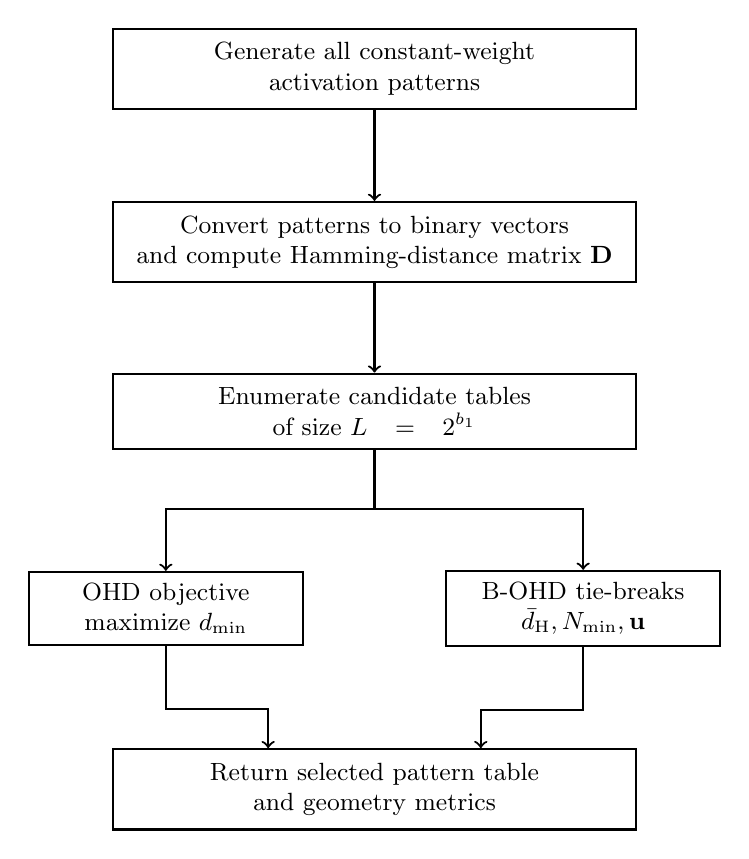
\begin{tikzpicture}[
        block/.style={
            rectangle,
            draw,
            thick,
            align=center,
            text width=6.3cm,
            minimum height=0.9cm,
            font=\small,
            inner sep=5pt
        },
        smallblock/.style={
            rectangle,
            draw,
            thick,
            align=center,
            text width=3.2cm,
            minimum height=0.85cm,
            font=\small,
            inner sep=4pt
        },
        arrow/.style={->, thick}
    ]

        \node[block] (all) at (0,0) {Generate all constant-weight\\activation patterns};
        \node[block] (bin) at (0,-2.20) {Convert patterns to binary vectors\\and compute Hamming-distance matrix \(\mathbf{D}\)};
        \node[block] (sets) at (0,-4.35) {Enumerate candidate tables\\of size \(L=2^{b_1}\)};
        \node[smallblock] (ohd) at (-2.65,-6.85) {OHD objective\\maximize \(d_{\min}\)};
        \node[smallblock] (bohd) at (2.65,-6.85) {B-OHD tie-breaks\\\(\bar{d}_{\mathrm{H}}, N_{\min}, \mathbf{u}\)};
        \node[block] (map) at (0,-9.15) {Return selected pattern table\\and geometry metrics};

        \draw[arrow] (all.south) -- (bin.north);
        \draw[arrow] (bin.south) -- (sets.north);
        \draw[arrow] (sets.south) -- ++(0,-0.75) -| (ohd.north);
        \draw[arrow] (sets.south) -- ++(0,-0.75) -| (bohd.north);
        \draw[arrow] (ohd.south) -- ++(0,-0.80) -| ([xshift=-1.35cm]map.north);
        \draw[arrow] (bohd.south) -- ++(0,-0.80) -| ([xshift=1.35cm]map.north);

    \end{tikzpicture}
    \caption{Pattern-selection flow for OHD and Balanced-OHD}
    \label{fig:ohd_balanced_pattern_selection_flow}
\end{figure}

The purpose of B-OHD is not to claim that carrier balance always dominates the pure OHD choice. Instead, it provides a controlled extension of OHD when multiple tables share the same minimum Hamming distance. This is why Chapter 5 reports OHD and B-OHD separately. If both methods select equivalent or nearly equivalent pattern tables for a given \((n,k)\), their BER curves may overlap. Such a result is not a failure of the method; it means that the selected pattern geometries are effectively the same under that configuration.

\subsubsection{Interpretation of the Pattern-Selection Outputs}

The pattern-selection stage produces more than the selected activation table. It also produces geometry indicators that help explain the BER results in Chapter 5. The most important indicator is \(d_{\min}\), because it describes the closest pair of patterns in the selected table. A larger \(d_{\min}\) generally means that a larger number of position-level mistakes is required before one valid index label can be confused with another.

The average Hamming distance \(\bar{d}_{\mathrm{H}}\) provides a complementary view. While \(d_{\min}\) focuses on the worst-separated pair, the average distance describes the overall separation of the selected table. Two tables can have the same \(d_{\min}\) but different average distances. In that case, B-OHD may prefer the table whose patterns are more separated on average, even if the worst-case pair is unchanged.

The number of closest pairs \(N_{\min}\) is also useful. If many pattern pairs achieve the minimum distance, the receiver has many vulnerable pattern confusions. If only one or two pairs are at the minimum distance, the weak part of the table is more localized. This distinction can affect the pattern error rate, especially at moderate SNR values where the MP probability map is informative but not yet fully reliable.

Finally, the carrier-usage vector \(\mathbf{u}\) indicates whether some local positions are used much more frequently than others. Strong imbalance is not always harmful by itself, but it may make the selected table less robust when certain positions have less reliable probability estimates. The balance metrics in B-OHD therefore serve as secondary tie-breakers, not as replacements for Hamming-distance separation.

\begin{table}[H]
\centering
\caption{Interpretation of pattern-selection criteria.}
\label{tab:pattern_selection_criteria_interpretation}
\begin{tabularx}{0.95\linewidth}{|p{3.2cm}|X|}
\hline
\textbf{Criterion} & \textbf{Interpretation in OTFS-IM detection} \\
\hline
\(d_{\min}\) & Worst-case separation between selected activation patterns; directly related to the most vulnerable pattern confusion. \\
\hline
\(\bar{d}_{\mathrm{H}}\) & Average geometric separation of the selected table; useful when several tables share the same \(d_{\min}\). \\
\hline
\(N_{\min}\) & Number of pattern pairs at the minimum distance; fewer closest pairs means fewer weakest confusions. \\
\hline
\(J_{\mathrm{var}}\), \(J_{\mathrm{span}}\) & Balance of local resource usage across the selected table; used only as secondary tie-breakers in B-OHD. \\
\hline
Random baseline & Diagnostic reference for checking whether deterministic table selection is actually beneficial. \\
\hline
\end{tabularx}
\end{table}

This interpretation is important because a lower total BER should not be attributed to OHD or B-OHD blindly. The selected table must also be examined through its geometry. If the selected tables have the same \(d_{\min}\), similar average distance, and similar carrier-usage statistics, then similar BER behavior is expected. Conversely, if one table has a clearly better distance profile, improvement in pattern error rate and index BER becomes more meaningful.

\subsubsection{Search Complexity and Random Diagnostic Baseline}

The exact OHD and B-OHD implementations enumerate all possible pattern tables of size \(L\) from \(\binom{n}{k}\) candidates. The number of candidate tables is
\begin{equation}
    N_{\mathrm{set}}
    =
    \binom{\binom{n}{k}}{L}.
    \label{eq:pattern_search_complexity}
\end{equation}
This search is acceptable for the small and moderate IM configurations used in this thesis, but it grows rapidly as \(n\) and \(k\) increase. For this reason, the implementation includes a guard condition that stops the exact search when the number of candidate tables exceeds a practical threshold. This keeps the simulation workflow focused on interpretable thesis configurations rather than on large-scale combinatorial optimization.

The simulation framework also includes a random-pattern diagnostic baseline. This baseline does not represent a proposed method. Its role is to test whether the deterministic pattern-selection rule provides a meaningful advantage over arbitrary valid pattern tables. In other words, random selection is used as an evaluation tool, not as a final design choice. If OHD or B-OHD gives lower pattern error rate and index BER than the random average, the result supports the claim that pattern geometry matters. If the random average is similar or better in some configurations, the result must be reported honestly and interpreted as a limitation of pure distance-based pattern selection for that configuration.

This distinction is important for the final evaluation. The baseline OTFS curve shows the effect of adding index modulation to OTFS. The OHD and B-OHD curves show the effect of deterministic pattern-table design inside OTFS-IM. The random-pattern curve, when enabled, checks whether the observed behavior is genuinely caused by the proposed table design or merely by the use of any valid activation-pattern subset.


\subsection{Design Discussion and Chapter Summary}

This section summarizes the OTFS-IM design developed in this chapter and clarifies how it will be evaluated in Chapter 5. The purpose is not to introduce another processing block, but to connect the design choices into one coherent interpretation: OTFS-IM changes the information mapping in the delay-Doppler domain, while OHD and B-OHD change the geometry of the activation-pattern table used by that mapping.

\subsubsection{Summary of the OTFS-IM Design Chain}

The implemented OTFS-IM system is built as an extension of the baseline OTFS transceiver described in Chapter 3. The baseline OTFS modulation and demodulation blocks are reused. The main modification is introduced before OTFS modulation, where the full delay-Doppler QAM grid is replaced by a sparse index-modulated grid. In each IM block, \(b_1\) bits select an activation pattern and \(b_2\) bits select the QAM symbols transmitted on the active positions.

This structure gives OTFS-IM two information-bearing mechanisms. The first one is conventional symbol modulation, represented by the QAM symbols placed on active delay-Doppler positions. The second one is index modulation, represented by the locations of those active positions. Therefore, the receiver cannot simply demodulate QAM symbols independently. It must also infer which activation pattern was transmitted in each block. This is why the MP detector is used to produce soft probability information, and a block-wise MAP stage is then applied to jointly recover index bits and symbol bits.

Table~\ref{tab:chapter4_design_summary} summarizes the main design elements introduced in this chapter and their roles in the implemented simulation model.

\begin{table}[H]
    \centering
    \caption{Summary of the implemented OTFS-IM design elements}
    \label{tab:chapter4_design_summary}
    \begin{tabularx}{\linewidth}{>{\RaggedRight\arraybackslash}p{3.2cm}
                                  >{\RaggedRight\arraybackslash}X
                                  >{\RaggedRight\arraybackslash}p{3.2cm}}
        \toprule
        Design element & Role in the OTFS-IM system & Main evaluation aspect \\
        \midrule
        IM block \((n,k)\) &
        Defines how many positions are available and how many of them are active in each block. &
        Spectral efficiency and sparsity level \\
        \midrule
        Activation-pattern table \(\mathcal{P}\) &
        Maps index bits to valid activation patterns and constrains the receiver MAP search. &
        Pattern error rate and index BER \\
        \midrule
        Power normalization \(\alpha\) &
        Compensates for the fact that only \(k\) out of \(n\) positions carry active QAM symbols. &
        Fairness of BER comparison \\
        \midrule
        MP probability output &
        Provides soft probabilities for QAM symbols and the inactive zero state. &
        Reliability of block-wise decisions \\
        \midrule
        Block-wise MAP decision &
        Recovers the most likely activation pattern and active QAM symbols per IM block. &
        Total BER, index BER, symbol BER \\
        \midrule
        OHD and B-OHD selection &
        Select deterministic pattern tables based on Hamming-distance geometry and balance criteria. &
        Pattern reliability and random baseline validation \\
        \bottomrule
    \end{tabularx}
\end{table}

The most important point from Table~\ref{tab:chapter4_design_summary} is that OTFS-IM is not only a modulation-rate modification. It changes the error structure of the receiver. A wrong activation pattern produces index-bit errors and may also place detected QAM symbols in the wrong positions. For this reason, the simulation study must report more than total BER. The separate index BER, symbol BER, and pattern error rate are necessary to explain why one configuration performs better or worse than another.

\subsubsection{BER-SE Trade-Off and Pattern Reliability}

The use of index modulation creates a trade-off between spectral efficiency and reliability. For one IM block, the number of transmitted bits is \(b_1+b_2\), while the block occupies \(n\) delay-Doppler positions. Thus, the spectral efficiency of the OTFS-IM mapping is controlled by the block parameters \((n,k)\):
\begin{equation}
    \eta_{\mathrm{IM}}
    =
    \frac{b_1+b_2}{n}.
    \label{eq:chapter4_im_se_summary}
\end{equation}
Increasing the number of active positions generally increases the number of QAM symbol bits, while changing \(n\) and \(k\) also changes the number of index bits. However, a higher spectral efficiency does not automatically imply a better system. If the chosen patterns are difficult to distinguish, the additional index bits may increase the error rate.

This is the reason OHD and B-OHD are included in the design. Their purpose is to make the activation patterns more distinguishable. The OHD method focuses on the minimum Hamming distance between selected patterns, while B-OHD additionally considers average distance, the number of closest pairs, and carrier-usage balance. These criteria are not expected to remove all detection errors, especially at low SNR where the MP detector itself may produce uncertain probability estimates. Instead, they aim to reduce pattern confusion when the receiver has enough information to benefit from a better pattern geometry.

Therefore, the final evaluation should be read in two layers. The first layer compares baseline OFDM-LMMSE, baseline OTFS, and OTFS-IM to show the effect of moving from conventional multicarrier transmission to delay-Doppler modulation and then to index modulation. The second layer compares OHD, B-OHD, and the random-pattern diagnostic baseline to show whether deterministic pattern selection improves the reliability of OTFS-IM. If a random pattern table performs close to or better than OHD in some configuration, that result should not be hidden. It indicates that minimum-distance selection alone is not always sufficient and that the benefit of OHD depends on the selected \((n,k)\) setting.

\subsubsection{Quantities to Track in the OTFS-IM Evaluation}

Because OTFS-IM has both symbol-domain and index-domain information, the simulation must track several quantities at the same time. These quantities are not interchangeable. Spectral efficiency explains how many bits are transmitted per delay-Doppler resource element, total BER describes end-to-end bit reliability, and pattern error rate describes whether the receiver selected the correct activation pattern. If only one of these quantities is reported, the behavior of the system can be misinterpreted.

\begin{table}[H]
\centering
\caption{Main quantities used to interpret OTFS-IM results.}
\label{tab:otfs_im_evaluation_quantities}
\begin{tabularx}{0.95\linewidth}{|p{3.0cm}|X|}
\hline
\textbf{Quantity} & \textbf{Reason for reporting} \\
\hline
\(\eta_{\mathrm{IM}}\) & Shows whether an OTFS-IM configuration is rate-fair with baseline OTFS or belongs to a lower-rate reliability-oriented setting. \\
\hline
\(\mathrm{BER}_{\mathrm{IM}}\) & Measures the final end-to-end bit error probability after both index and symbol bits are reconstructed. \\
\hline
\(\mathrm{BER}_{\mathrm{idx}}\) & Isolates errors caused by incorrect recovery of the activation-pattern label. \\
\hline
\(\mathrm{BER}_{\mathrm{sym}}\) & Isolates errors in the QAM symbol bits on positions detected as active. \\
\hline
\(\mathrm{PER}_{\mathrm{pat}}\) & Measures block-level activation-pattern confusion, which is directly affected by pattern-table geometry. \\
\hline
\end{tabularx}
\end{table}

Table~\ref{tab:otfs_im_evaluation_quantities} is also useful for avoiding an overly simple conclusion. A configuration may have low total BER because it transmits fewer bits per block. Another configuration may have higher BER but preserve the same spectral efficiency as baseline OTFS. Similarly, a pattern table may reduce pattern error rate while the total BER remains limited by QAM symbol errors. The evaluation in Chapter 5 is therefore designed to connect these quantities rather than judge the system from a single curve.

\subsubsection{Connection to Chapter 5 Simulation Results}

The design in this chapter directly determines the structure of the simulation results in Chapter 5. The BER overview figure compares OFDM-LMMSE, baseline OTFS, OHD OTFS-IM, and B-OHD OTFS-IM under the same channel and SNR settings. The OTFS-IM error-decomposition figure then separates total BER into index BER, symbol BER, and pattern error rate so that the source of the errors can be identified. The pattern-geometry figure connects the selected activation table to Hamming-distance and carrier-usage properties. Finally, the random-pattern validation figure checks whether the proposed deterministic tables are actually better than arbitrary valid pattern selections.

This evaluation structure follows directly from the design logic of the chapter. If OTFS-IM improves BER at a comparable or higher spectral efficiency, the result supports the usefulness of index modulation in the delay-Doppler domain. If OHD or B-OHD reduces pattern error rate or index BER compared with random selection, the result supports the importance of pattern geometry. If the improvement is small or configuration-dependent, the result still has value because it identifies the limitation of the selected pattern design and motivates further work on detector-aware or channel-aware pattern selection.

In summary, this chapter has developed the OTFS-IM system used in the thesis simulations. It defined the IM block structure, spectral-efficiency expression, activation-pattern mapping, transmitter and receiver processing chains, block-wise MAP recovery, and the OHD/B-OHD pattern-selection methods. These elements provide the technical foundation for Chapter 5, where the proposed OTFS-IM design is evaluated through BER performance, error decomposition, pattern reliability, and BER-SE trade-off analysis.

\newpage


\newpage
